\documentclass[conference]{IEEEtran}

\usepackage{amsmath,amssymb,mathtools}
\usepackage{graphicx}
\usepackage{booktabs,tabularx,array}
\usepackage{algorithm}
\usepackage{algorithmic}
\usepackage{cite}
\usepackage{url}

% Generated by make_paper_numbers.py from results_manifest.json folders.
% Do not edit: every value is re-derived from the result CSVs.
\newcommand{\AlgThreeA}{106.6}
\newcommand{\AlgThreeASD}{7.6}
\newcommand{\AlgThreeB}{165.1}
\newcommand{\AlgThreeBSD}{12.1}
\newcommand{\AlgThreeBtwo}{168.6}
\newcommand{\AlgThreeBtwoSD}{16.4}
\newcommand{\AlgThreeC}{168.6}
\newcommand{\AlgThreeCSD}{16.4}
\newcommand{\AlgThreeWA}{0.0}
\newcommand{\AlgThreeWASD}{0.0}
\newcommand{\CpuMaxA}{92.5}
\newcommand{\CpuMaxASD}{23.0}
\newcommand{\CpuMaxB}{19.9}
\newcommand{\CpuMaxBSD}{8.7}
\newcommand{\CpuMaxBtwo}{22.9}
\newcommand{\CpuMaxBtwoSD}{2.7}
\newcommand{\CpuMaxC}{7.6}
\newcommand{\CpuMaxCSD}{1.2}
\newcommand{\CpuMaxWA}{147.2}
\newcommand{\CpuMaxWASD}{48.2}
\newcommand{\CpuRepeatMedianA}{98.6}
\newcommand{\CpuRepeatMedianC}{7.4}
\newcommand{\CpuRepeatRedMax}{93}
\newcommand{\CpuRepeatRedMin}{92}
\newcommand{\CpuTotalA}{92.5}
\newcommand{\CpuTotalASD}{23.0}
\newcommand{\CpuTotalB}{19.9}
\newcommand{\CpuTotalBSD}{8.7}
\newcommand{\CpuTotalBtwo}{22.9}
\newcommand{\CpuTotalBtwoSD}{2.7}
\newcommand{\CpuTotalC}{21.9}
\newcommand{\CpuTotalCSD}{2.0}
\newcommand{\CpuTotalWA}{147.2}
\newcommand{\CpuTotalWASD}{48.2}
\newcommand{\FleetTardBSixteen}{117,682}
\newcommand{\FleetTardBTwenty}{122,279}
\newcommand{\FleetTardBtwoSixteen}{90,343}
\newcommand{\FleetTardBtwoTwenty}{90,104}
\newcommand{\GanttLongWaitA}{6,737.3}
\newcommand{\GanttLongWaitAgvA}{AGV-20}
\newcommand{\GanttPanelAImbalance}{6,734.6}
\newcommand{\GanttPanelALastDelivery}{7,547.5}
\newcommand{\GanttPanelAWaitTotal}{62,169.9}
\newcommand{\GanttPanelCImbalance}{1,503.8}
\newcommand{\GanttPanelCLastDelivery}{2,549.8}
\newcommand{\GanttPanelCWaitTotal}{26,293.1}
\newcommand{\GanttSameAgvWaitC}{375.0}
\newcommand{\GanttServiceSameAgv}{160.0}
\newcommand{\GanttZoomAgv}{AGV-03}
\newcommand{\GanttZoomLiftTrips}{10}
\newcommand{\GanttZoomLobbyWaitTotal}{1,179.5}
\newcommand{\GanttZoomLobbyWaits}{12}
\newcommand{\GiniC}{0.143}
\newcommand{\GiniCRotate}{0.145}
\newcommand{\ImbalanceA}{7,149.9}
\newcommand{\ImbalanceASD}{772.6}
\newcommand{\ImbalanceB}{2,832.3}
\newcommand{\ImbalanceBSD}{291.4}
\newcommand{\ImbalanceBtwo}{1,441.2}
\newcommand{\ImbalanceBtwoSD}{241.1}
\newcommand{\ImbalanceC}{1,441.2}
\newcommand{\ImbalanceCSD}{241.1}
\newcommand{\ImbalanceWA}{5,144.8}
\newcommand{\ImbalanceWASD}{488.2}
\newcommand{\MakespanA}{7,972.4}
\newcommand{\MakespanASD}{819.1}
\newcommand{\MakespanB}{3,705.9}
\newcommand{\MakespanBSD}{309.8}
\newcommand{\MakespanBtwo}{2,768.9}
\newcommand{\MakespanBtwoSD}{195.8}
\newcommand{\MakespanC}{2,768.9}
\newcommand{\MakespanCSD}{195.8}
\newcommand{\MakespanWA}{5,999.9}
\newcommand{\MakespanWASD}{526.5}
\newcommand{\MessagesA}{0.0}
\newcommand{\MessagesASD}{0.0}
\newcommand{\MessagesB}{0.0}
\newcommand{\MessagesBSD}{0.0}
\newcommand{\MessagesBtwo}{337.2}
\newcommand{\MessagesBtwoSD}{16.2}
\newcommand{\MessagesC}{337.2}
\newcommand{\MessagesCSD}{16.2}
\newcommand{\MessagesWA}{0.0}
\newcommand{\MessagesWASD}{0.0}
\newcommand{\RedAlgThreeCA}{+58}
\newcommand{\RedCpuMaxCA}{-92}
\newcommand{\RedCpuMaxCAabs}{92}
\newcommand{\RedCpuTotalCA}{-76}
\newcommand{\RedCpuTotalCAabs}{76}
\newcommand{\RedImbalanceCA}{-80}
\newcommand{\RedImbalanceCAabs}{80}
\newcommand{\RedMakespanCA}{-65}
\newcommand{\RedMakespanCAabs}{65}
\newcommand{\RedTardinessCA}{-72}
\newcommand{\RedTardinessCAabs}{72}
\newcommand{\RedWaitMaxCA}{-74}
\newcommand{\RedWaitMaxCAabs}{74}
\newcommand{\RedWaitTotalCA}{-58}
\newcommand{\RedWaitTotalCAabs}{58}
\newcommand{\RedWindowsMaxCA}{-69}
\newcommand{\RedWindowsMaxCAabs}{69}
\newcommand{\SeedSevenCpuCentralA}{92.8}
\newcommand{\SeedSevenCpuCentralC}{7.7}
\newcommand{\SeedSevenCpuFloorOneC}{3.6}
\newcommand{\SeedSevenCpuFloorThreeC}{5.2}
\newcommand{\SeedSevenCpuFloorTwoC}{7.4}
\newcommand{\SeedSevenLargestCCpu}{7.4}
\newcommand{\SeedSevenLargestCWindows}{619}
\newcommand{\SeedSevenLastDeliveryA}{7,547.5}
\newcommand{\SeedSevenWindowsCentralA}{1,989}
\newcommand{\SeedSevenWindowsCentralC}{146}
\newcommand{\SeedSevenWindowsFloorOneC}{478}
\newcommand{\SeedSevenWindowsFloorThreeC}{454}
\newcommand{\SeedSevenWindowsFloorTwoC}{619}
\newcommand{\SensitivityRows}{324}
\newcommand{\TardinessA}{316,893.6}
\newcommand{\TardinessASD}{41,316.3}
\newcommand{\TardinessB}{122,278.8}
\newcommand{\TardinessBSD}{11,430.7}
\newcommand{\TardinessBtwo}{90,104.5}
\newcommand{\TardinessBtwoSD}{11,447.3}
\newcommand{\TardinessC}{90,104.5}
\newcommand{\TardinessCSD}{11,447.3}
\newcommand{\TardinessWA}{226,879.9}
\newcommand{\TardinessWASD}{22,351.3}
\newcommand{\WAImbalance}{5,144.8}
\newcommand{\WAMakespan}{5,999.9}
\newcommand{\WATardiness}{226,879.9}
\newcommand{\WaitMaxA}{7,133.4}
\newcommand{\WaitMaxASD}{817.9}
\newcommand{\WaitMaxB}{2,830.8}
\newcommand{\WaitMaxBSD}{302.2}
\newcommand{\WaitMaxBtwo}{1,887.7}
\newcommand{\WaitMaxBtwoSD}{173.9}
\newcommand{\WaitMaxC}{1,887.7}
\newcommand{\WaitMaxCSD}{173.9}
\newcommand{\WaitMaxWA}{5,133.9}
\newcommand{\WaitMaxWASD}{487.8}
\newcommand{\WaitTopA}{0.0}
\newcommand{\WaitTopC}{1,169.1}
\newcommand{\WaitTotalA}{64,689.7}
\newcommand{\WaitTotalASD}{8,466.2}
\newcommand{\WaitTotalB}{27,647.7}
\newcommand{\WaitTotalBSD}{2,747.6}
\newcommand{\WaitTotalBtwo}{27,104.5}
\newcommand{\WaitTotalBtwoSD}{2,180.2}
\newcommand{\WaitTotalC}{27,104.5}
\newcommand{\WaitTotalCSD}{2,180.2}
\newcommand{\WaitTotalWA}{49,584.5}
\newcommand{\WaitTotalWASD}{4,778.5}
\newcommand{\WindowsMaxA}{2,030.7}
\newcommand{\WindowsMaxASD}{84.5}
\newcommand{\WindowsMaxB}{1,733.5}
\newcommand{\WindowsMaxBSD}{69.5}
\newcommand{\WindowsMaxBtwo}{1,733.5}
\newcommand{\WindowsMaxBtwoSD}{69.5}
\newcommand{\WindowsMaxC}{634.5}
\newcommand{\WindowsMaxCSD}{30.0}
\newcommand{\WindowsMaxWA}{2,075.8}
\newcommand{\WindowsMaxWASD}{84.4}


\title{Hierarchical Hybrid Planning for Multi-AGV Scheduling in Multi-Floor Factories}

\author{\IEEEauthorblockN{[AUTHORS]}\IEEEauthorblockA{[AFFILIATION]}\\
\IEEEauthorblockA{[EMAIL]}}

\begin{document}
\maketitle

\begin{abstract}
Multi-floor manufacturing requires automated guided vehicles (AGVs) to share both floor routes and lift resources. We extend the prioritized planning baseline of Guo et al. (ICARCV 2024) with a hybrid architecture: a central server assigns jobs, splits routes at lifts, and books lift trips, while one server per floor plans local route legs. Lift-lobby waiting points let delays be absorbed near floor-level conflicts instead of at the factory's single parking node. In the tested three-floor layout (27 nodes, 4 lifts), ten job sets of 100 jobs and 20 AGVs, the hybrid configuration reduces mean last-delivery makespan by \RedMakespanCAabs\%, total tardiness by \RedTardinessCAabs\%, and load imbalance by \RedImbalanceCAabs\% relative to the paper-style centralized configuration, with busiest-server CPU down \RedCpuMaxCAabs\%. All reported plans pass an independent verifier. These are experimental results for the tested layout and settings, not a general optimality or scalability guarantee.
\end{abstract}

\begin{IEEEkeywords}
Automated guided vehicles, multi-agent path finding, prioritized planning, multi-floor logistics, lift coordination, hierarchical scheduling.
\end{IEEEkeywords}

\section{Introduction}
\label{sec:intro}

Automated guided vehicles (AGVs) are a central part of material handling in smart manufacturing, moving workpieces between storage, processing, and delivery locations. Coordinating a fleet is a joint assignment, routing, and traffic-management problem: vehicles may need the same narrow aisle, workstation approach, or transport resource at overlapping times. A schedule must assign jobs and produce routes and timings that avoid collisions while meeting operational targets such as completion time, delivery due dates, and balanced vehicle utilization.

These requirements become more demanding in multi-floor facilities, where lifts connect otherwise separate floor networks. A lift is a shared resource with finite capacity and non-negligible travel time: a conflict at one lift can delay routes on several floors and propagate through the entire schedule. The prioritized planning baseline of Guo et al. \cite{guo2024} assigns transport tasks and plans routes sequentially by AGV priority, resolving conflicts against previously planned higher-priority vehicles. In that baseline, however, AGVs may wait only at the factory's single parking node. With lifts, the next available floor leg may be blocked by traffic on another floor, and parking-node-only waiting can serialize delays that would be better absorbed near the lift itself.

This paper extends the prioritized-planning baseline with a hybrid architecture for a multi-floor factory. A central server performs job assignment, divides each AGV route into floor-level legs at lift edges, and books lift trips, which remain shared across floors and therefore require system-wide coordination. One edge server per floor plans local route legs using prioritized conflict-free routing, and lift-lobby waiting points let a floor server delay a leg at its entry lobby instead of returning the AGV to parking. Job assignment, lift booking, dispatch, merging, and verification stay centrally orchestrated; the floor servers do not negotiate with each other directly.

The implementation is evaluated against the paper-style centralized configuration (waiting at parking only) and a centralized variant with the same lift lobbies, on ten job sets of 100 jobs and 20 AGVs in a tested three-floor layout with 27 nodes and 4 lifts. Every generated plan passes an independent verifier. The hybrid configuration reduces mean last-delivery makespan by \RedMakespanCAabs\%, total tardiness by \RedTardinessCAabs\%, and load imbalance by \RedImbalanceCAabs\% relative to the paper-style centralized configuration; its busiest-server planning CPU time falls by \RedCpuMaxCAabs\%. These figures describe the tested factory, parameters, and seeds, not general guarantees for all multi-floor factories.

The three narrow contributions are: (i) a corrected reimplementation of the ICARCV 2024 prioritized-planning baseline with independent full-plan verification; (ii) a hybrid central-plus-floor-server architecture that separates central job assignment and lift booking from per-floor route-leg planning; and (iii) lift-lobby waiting points that absorb delays near floor-level conflicts and lift resources.

The remainder is organized as follows. Section~\ref{sec:related} reviews directly related work; Section~\ref{sec:model} defines the scheduling model; Section~\ref{sec:method} describes the algorithms and the hybrid extension; Section~\ref{sec:experiments} reports the setup and results; Section~\ref{sec:conclusion} concludes and states limitations.

\section{Related Work}
\label{sec:related}

Guo et al.'s ICARCV 2024 method is the baseline for this study: large-scale multiple-AGV scheduling as prioritized assignment and route planning, resolving conflicts against previously planned higher-priority vehicles \cite{guo2024}. The sequential approach avoids joint search over all vehicle paths, but its result depends on assignment and priority order.

Prioritized wait adjustment starts from individual paths and shifts waiting using safe intervals; its preliminary evaluation reports 50--250 agents and trades solution quality for runtime \cite{andreychuk2018}. It is our competing planner (WA) in Section~\ref{sec:experiments}.

Conflict-based search (CBS) offers a coupled alternative. Continuous-time CBS methods model nonuniform action durations and geometric collisions \cite{andreychuk2022}; He et al. extend CBS to multi-floor MAPF with single-agent elevator occupancy and reset intervals, explicitly including lift conflicts in search \cite{he2026}. These methods provide stronger conflict reasoning, while our experiments focus on job assignment, prioritized route windows, and lift arbitration in a decomposed planner.

Optimization-based heuristics scale to larger fleets: Hu et al. use reservation timetables with variable-neighborhood search on 3--200 AGVs \cite{hu2022}, and Verma et al. allow multiple reservations at shared resource points \cite{verma2024}. At very high scale, MAPF-LNS2 repairs colliding subsets of agents and has solved warehouse instances with up to 8,000 agents \cite{mapflns2022}, though its warehouse experiments do not model lifts as a constrained resource.

Hierarchical and zone-based planning motivates layered coordination: the spare-zone method of Zhao et al. uses a hierarchical allocation layer and local coordination for vehicles following fixed paths \cite{zhao2021}; Pratissoli et al. use a centralized, decoupled, multilayer traffic manager with topological sectors \cite{pratissoli2024}; HMAPP combines high-level region sequences with regional conflict-based searches \cite{hmapp2021}. The present implementation instead partitions local route windows by floor while retaining central job assignment and lift booking.

\section{Problem Model}
\label{sec:model}

The model uses the prioritized assignment and route-window notation of the ICARCV baseline \cite{guo2024}, with explicit lift and lobby elements for a multi-floor factory.

\subsection{Sets and graph}
Let $G=(N,E)$ be the undirected factory graph. Each undirected edge represents a bidirectional track. Let $F$ be the set of floors, $N_f\subseteq N$ the nodes on floor $f\in F$, and $L\subseteq E$ the set of lift links between floors. The parking node is $\pi\in N$. Let $J$ be the set of jobs and $V$ the set of AGVs; each job is served by exactly one AGV. Let $M_i$ index the successive node visits on AGV $i$'s route, including repeated visits to the same physical node.

\subsection{Parameters}
Each job $j\in J$ has pickup and delivery nodes $p_j,p'_j\in N$ ($p_j\ne p'_j$) and desired times $t_j,t'_j$. Service times are $\eta$ (loading) and $\eta'$ (unloading); safety separation is $\delta>0$; AGV speed is $v>0$. Each edge $e\in E$ has length $\ell_e$; for lift edges, $\ell_e$ is the configured lift length. Travel time along an edge is $\tau_{uv}=\ell_{\{u,v\}}/v$, and $d(u,w)$ is shortest-path travel time. Jobs are considered in increasing desired pickup time $(t_j,j)$; AGV $i$ has fixed priority rank $\rho_i$ (smaller means higher priority). Assignment uses fitness weight $\lambda\ge0$ and Algorithm 3 is limited to $k_{\max}$ passes.

\subsection{Decision and schedule variables}
The assignment variable is $x_{ji}\in\{0,1\}$, where $x_{ji}=1$ means AGV $i$ is assigned job $j$: $\sum_{i\in V}x_{ji}=1\ \forall j\in J$. For each AGV $i$, $R_i=(n_{i,0},\ldots,n_{i,q_i})$ is its ordered route with $n_{i,0}=n_{i,q_i}=\pi$, constructed by concatenating shortest paths through each assigned job's pickup and delivery nodes and back to $\pi$. For visit $m$, $lt_{im}$ and $rt_{im}$ are the start and end of its node-occupancy window; dwell equals $\eta$ at pickup, $\eta'$ at delivery, and zero at pass-through visits. The edge window for consecutive visits is $[rt_{i,m-1},lt_{im}]$ with fixed duration $\tau_{n_{i,m-1},n_{i,m}}$: the AGV does not stop while traversing an edge.

\subsection{Assignment quantities}
When job $j$ is considered, with AGV $i$'s current node $s_i$ and available time $vt_i$:
\begin{align*}
  ct_{ji} &= vt_i + d(s_i,p_j) + \eta + d(p_j,p'_j) + \eta',\\
  et_{ji} &= \max\!\left(0,\ t_j-\bigl(vt_i+d(s_i,p_j)+\eta\bigr)\right),\\
  dt_{ji} &= \max(0,\ ct_{ji}-t'_j),\\
  F_{ji} &= ct_{ji}+\lambda(et_{ji}+dt_{ji}).
\end{align*}
The job is assigned to the AGV minimizing $F_{ji}$ (ties by priority); then $vt_i$ and $s_i$ are updated to $ct_{ji}$ and $p'_j$.

\subsection{Conflict separation}
Let $W_n$ be fixed occupancy windows of higher-priority AGVs at ordinary node $n$, and $W'_{uv}$ fixed edge windows on directed traversal $u\to v$ (a physical track is exclusive in both directions). Overlapping use of an ordinary node or the same bidirectional track by distinct AGVs must be separated by at least $\delta$: for intervals $[a,b]$ and $[c,d]$, require $c\ge b+\delta$ or $a\ge d+\delta$. The parking node is exempt from node separation. Algorithm 3 resolves a conflict by shifting a route prefix right by cumulative delay $st^*$ (sweep backward from the conflict visit to the nearest previous exempt node, limited to $k_{\max}$ passes), extending the preceding exempt node's window by $st^*$.

\subsection{Objectives}
Let $C_j$ be job $j$'s actual delivery-completion time and $U_i$ AGV $i$'s usage time (return time to $\pi$ when serving jobs). Then
\begin{align*}
  M &= \max_{j\in J} C_j &&\text{(makespan, last delivery)},\\
  T &= \sum_{j\in J}\max(0,C_j-t'_j) &&\text{(total delivery tardiness)},\\
  I &= \max_{i\in V}U_i-\min_{i\in V}U_i &&\text{(load imbalance)}.
\end{align*}
Possible objectives are $\min\;\alpha M+\beta T+\gamma I$ or lexmin$(M,T,I)$; the code does not optimize either combined objective, it reports $M,T,I$ as metrics.

\section{Method}
\label{sec:method}

The method combines the prioritized assignment and route-window procedures of the centralized baseline \cite{guo2024} with a hierarchical floor decomposition. A central server assigns jobs, splits routes at lifts, books lift trips, and merges plans; one edge server per floor plans local route legs.

Figure~\ref{fig:architecture} shows the information flow. Jobs and fleet state go to the central server; legs and reservations cross between central and floor servers; merged, verified schedules go to the AGVs for execution.

\subsection{Algorithms 1--3 recap}
Algorithm~\ref{alg:assignment} assigns jobs in order $(t_j,j)$ to the AGV minimizing $F_{ji}$. Algorithm~\ref{alg:routing} processes AGVs in priority order $V_1\to V_{|V|}$, constructing node and edge windows; a window conflicting with frozen reservations triggers Algorithm~\ref{alg:sliding}, which delays the affected route segment. Algorithm~\ref{alg:sliding} sweeps backward from the conflict visit to the nearest preceding exempt node, accumulating the smallest right-shift that clears higher-priority windows with separation $\delta$, up to $k_{\max}$ passes; on exhaustion it delays departure at the exempt node until blocking traffic clears.

\begin{algorithm}[t]
\caption{Prioritized job assignment (Algorithm 1)}
\label{alg:assignment}
\small
\begin{algorithmic}[1]
\REQUIRE Jobs $J$, AGVs $V$, fitness weight $\lambda$, service times $\eta,\eta'$
\ENSURE Assignment $x_{ji}$ and complete routes $R_i$
\FOR{each $j\in J$ in order $(t_j,j)$}
  \FOR{each $i\in V$}
    \STATE Compute $ct_{ji},et_{ji},dt_{ji}$ from AGV state $(s_i,vt_i)$.
    \STATE $F_{ji}\gets ct_{ji}+\lambda(et_{ji}+dt_{ji})$.
  \ENDFOR
  \STATE Choose $i^*\gets\arg\min_i(F_{ji},\rho_i)$; set $x_{ji^*}\gets1$.
  \STATE Append shortest paths $s_{i^*}\to p_j\to p'_j$ with dwell $\eta,\eta'$.
  \STATE Update AGV state to $(p'_j,ct_{ji^*})$.
\ENDFOR
\FOR{each $i\in V$}
  \STATE Append a shortest path from the final assigned station to $\pi$.
\ENDFOR
\end{algorithmic}
\end{algorithm}

\begin{algorithm}[t]
\caption{Prioritized conflict-free routing (Algorithm 2)}
\label{alg:routing}
\small
\begin{algorithmic}[1]
\REQUIRE Routes $R_i$, dwell times, priority order $V_1,\ldots,V_{|V|}$
\ENSURE Timed plans and frozen reservations $W_n,W'_e$
\STATE Initialize empty node and edge reservation sets $W_n,W'_e$.
\FOR{each AGV $i$ in priority order}
  \STATE Construct node and edge windows along $R_i$.
  \FOR{each candidate window conflicting with $W_n$ or $W'_e$}
    \STATE Apply Algorithm~\ref{alg:sliding} to delay the route segment.
  \ENDFOR
  \STATE Freeze ordinary node windows in $W_n$ and track windows in $W'_e$.
\ENDFOR
\end{algorithmic}
\end{algorithm}

\begin{algorithm}[t]
\caption{Sliding-window conflict elimination (Algorithm 3)}
\label{alg:sliding}
\small
\begin{algorithmic}[1]
\REQUIRE Conflict visit $p$, reservations $W$, route $R$, limit $k_{\max}$
\ENSURE Conflict-free shifted windows and delay $st^*$
\STATE Find the nearest preceding exempt visit $q$.
\FOR{$k=1$ to $k_{\max}$}
  \STATE Set $st^*\gets0$ and $mt^*\gets\infty$.
  \FOR{visits $m=p,p-1,\ldots,q+1$}
    \STATE Evaluate $f(lt_m+st^*,rt_m+st^*,W)$; update $mt^*$ and $st^*$.
    \IF{$st^*>mt^*$} \STATE Stop this backward sweep. \ENDIF
  \ENDFOR
  \IF{the sweep completes within $mt^*$} \STATE \textbf{break} \ENDIF
\ENDFOR
\IF{no feasible sweep completed}
  \STATE Apply the fallback delay at $q$ until blocking reservations clear.
\ENDIF
\STATE Shift windows $q+1,\ldots,p$ and extend the window at $q$ by $st^*$.
\end{algorithmic}
\end{algorithm}

\subsection{Hybrid central-plus-floor-server extension}
The hybrid planner cuts each complete route at lift edges into floor-local legs. Each floor server schedules its legs using local node and track reservations; when needed, the AGV waits at its entry lobby or at $\pi$. The central server reserves the lift track at the earliest available time after the AGV is ready, respecting safety separation, then releases the next floor leg at the arrival lobby. Floor and lift windows are merged into complete plans before independent verification.

Legs are dispatched either in priority order or first-come-first-served (FCFS): FCFS orders legs by release time, AGV priority, then leg index; priority order processes higher-priority AGVs' legs first and is used as a decomposition check. On the tested seeds, priority-order hybrid plans match the centralized-with-lobbies plans. Configuration C (the default hybrid) uses FCFS order.

\begin{algorithm}[t]
\caption{Hybrid floor-leg planning and lift booking}
\label{alg:hybrid}
\small
\begin{algorithmic}[1]
\REQUIRE Assigned routes, floor planners, central lift calendar, dispatch order
\ENSURE Merged complete AGV plans
\STATE Split each route into maximal floor-local legs at every lift.
\STATE Insert each initial leg into the dispatch queue using the chosen order.
\WHILE{the queue is nonempty}
  \STATE Remove the next leg and schedule it with its floor planner.
  \IF{the route continues on another floor}
    \STATE Reserve the intervening lift trip centrally.
    \STATE Release the next leg at the arrival lobby after lift travel.
  \ENDIF
\ENDWHILE
\STATE Merge floor-leg and lift windows; independently verify each plan.
\end{algorithmic}
\end{algorithm}

\begin{figure}[t]
\centering
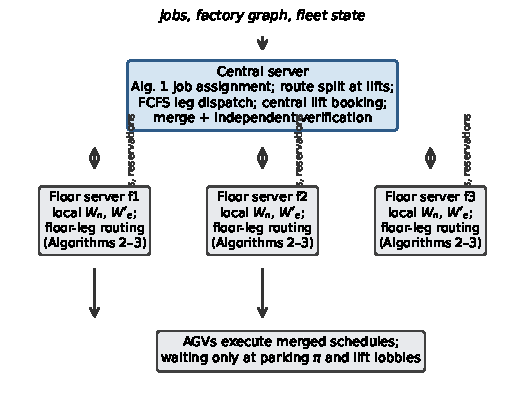
\includegraphics[width=\columnwidth]{../figures/architecture.pdf}
\caption{Hybrid architecture: central job assignment, route split, lift booking, and verification; per-floor route-leg planning; AGVs execute merged schedules, waiting only at parking $\pi$ and lift lobbies.}
\label{fig:architecture}
\end{figure}

\section{Experiments}
\label{sec:experiments}

\subsection{Setup}
Table~\ref{tab:setup} summarizes the layout, job model, planner parameters, and configurations. All configurations use $\eta=\eta'=16$~s, $\delta=10$~s, $\lambda=1.0$, and $v=1$~m/s; lift links use their configured 40~m length (40~s non-stop travel). The main comparison uses 100 jobs, 20 AGVs, seeds 1--10, and the strict track rule; the fleet sweep uses 4, 8, 12, 16, and 20 AGVs over the same job-generation settings. Every generated schedule is passed to an independent verifier that checks route endpoints, node and bidirectional-track separation, edge travel durations, dwell windows, and exactly-once job service; a run is accepted only when the verifier returns no violations.

\begin{table*}[t]
\centering
\small
\caption{Experimental setup (layout, job model, parameters, configurations).}
\label{tab:setup}
\resizebox{\textwidth}{!}{
\begin{tabular}{ll}
\toprule
Layout & 3 floors; 27 operational nodes (9 per floor); 38 edges; 4 lifts (40 m each); parking $\pi=$ 1A; 26 non-parking, non-lobby job stations \\
Jobs & pickup and delivery sampled uniformly from the 26 stations; $t_j\sim U[0,600]$ s; slack $s_j\sim U[30,200]$ s; $t'_j=t_j+d(p_j,p'_j)+\eta+\eta'+s_j$ \\
Fleet & 20 AGVs (\texttt{AGV-01}--\texttt{AGV-20}), fixed priorities $V_1$--$V_{20}$; fleet sweep: 4, 8, 12, 16, 20 AGVs \\
Parameters & $\eta=\eta'=16$~s; $\delta=10$~s; $\lambda=1.0$; $v=1$~m/s; lift travel 40~s \\
Main experiment & 100 jobs, 20 AGVs, seeds 1--10, strict track rule \\
Configurations & A: centralized paper-style (wait at parking only); B: centralized with lobbies; B2: centralized with lobbies and FCFS leg order; C: hybrid central + floor servers, lobbies, FCFS leg order \\
\bottomrule
\end{tabular}}
\end{table*}

\subsection{Main results: Gantt chart as main visual evidence}
Figure~\ref{fig:gantt-seed7} shows the A and C plans for seed 7 (100 jobs, 20 AGVs) on a shared time axis; rows are AGVs in priority order, colors are activities (moving on floor 1/2/3, lift trip, loading $\eta$, unloading $\eta'$), and hatched bars are waiting. Panel titles give data-derived totals. What to notice: under A the rows form a staircase of waiting that descends with priority. The annotation marks \GanttLongWaitAgvA{}: it waits \GanttLongWaitA~s before its first move under A but only \GanttSameAgvWaitC~s under C, while its service time is \GanttServiceSameAgv~s in both configurations — the same AGV's workload is unchanged, the waiting almost entirely disappears. Figure~\ref{fig:gantt-zoom} explains the hybrid: for \GanttZoomAgv{} (10 lift trips, floors 1--3), the route is cut into floor legs joined by lift trips, and the waiting between legs sits at lift lobbies rather than on floor nodes.

\begin{figure*}[t]
\centering
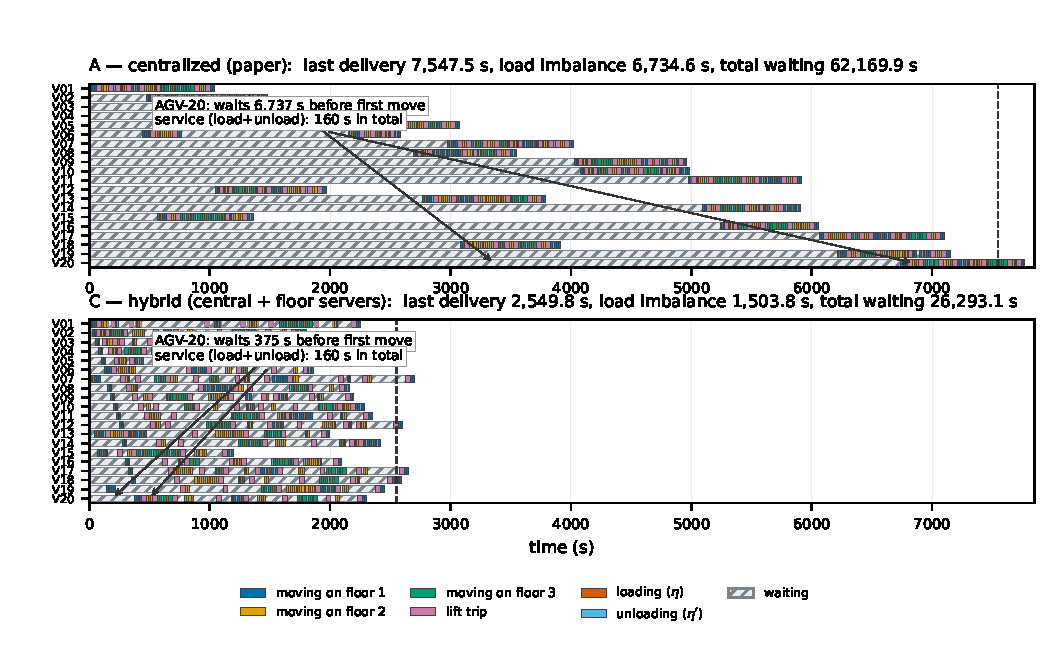
\includegraphics[width=\textwidth]{../figures/gantt_A_C_seed7.pdf}
\caption{How to read: each row is one AGV in priority order (V01 highest priority); colors are activities (moving on floor 1/2/3, lift trip, loading $\eta$, unloading $\eta'$); hatched bars are waiting. Panels show the seed-7 job set under A (top) and C (bottom) on a shared time axis; dashed vertical lines mark each panel's last delivery (the bars continue to the final return to parking). Under A the rows form a staircase of waiting that descends with priority. The annotation marks \GanttLongWaitAgvA{}: it waits \GanttLongWaitA~s before its first move under A but only \GanttSameAgvWaitC~s under C, while its service time is \GanttServiceSameAgv~s in both configurations. Panel titles give data-derived totals: last delivery \GanttPanelALastDelivery{} versus \GanttPanelCLastDelivery~s, load imbalance \GanttPanelAImbalance{} versus \GanttPanelCImbalance~s, total waiting \GanttPanelAWaitTotal{} versus \GanttPanelCWaitTotal~s.}
\label{fig:gantt-seed7}
\end{figure*}

\begin{figure}[t]
\centering
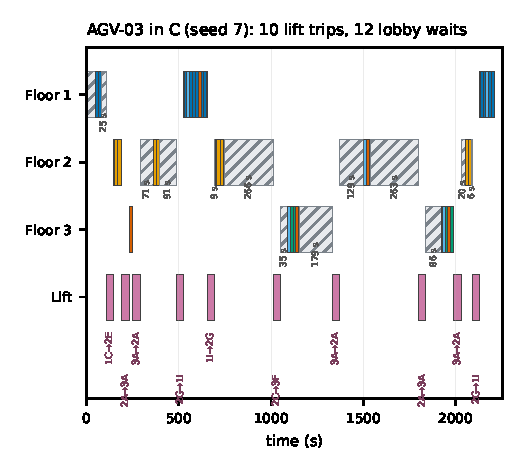
\includegraphics[width=\columnwidth]{../figures/gantt_zoom_seed7_agv-03.pdf}
\caption{How the hybrid builds one route, shown for \GanttZoomAgv{} on the same seed. Rows are the three floors and the lifts; the AGV's route is cut into floor legs joined by \GanttZoomLiftTrips{} lift trips (labelled with their lobby-to-lobby nodes). Hatched bars at lift-entry lobbies are lobby waits: \GanttZoomLobbyWaits{} waits totalling \GanttZoomLobbyWaitTotal~s. Between floor legs the AGV waits at lift lobbies rather than holding a floor node.}
\label{fig:gantt-zoom}
\end{figure}

Table~\ref{tab:mean-results} reports the ten-seed means with sample standard deviations. C reduces makespan by \RedMakespanCAabs\%, tardiness by \RedTardinessCAabs\%, and imbalance by \RedImbalanceCAabs\% relative to A. B2 and C have identical schedule outcomes on every seed, so the B2--C contrast isolates the floor-server split's computation/state distribution (server CPU \CpuMaxC~vs~\CpuMaxBtwo~ms at the busiest server; \MessagesC~central--floor messages) rather than a schedule-quality change.

\begin{table*}[t]
\centering
\small
\caption{Mean $\pm$ sample standard deviation over ten seeds (100 jobs, 20 AGVs). Percentages compare C with A. B2 and C have identical schedule outcomes on every seed, so B2 is omitted from the columns.}
\label{tab:mean-results}
\resizebox{\textwidth}{!}{
\begin{tabular}{lrrrr}
\toprule
Metric & A & B & C & C vs. A \\
\midrule
Last-delivery makespan (s) & $\MakespanA\pm\MakespanASD$ & $\MakespanB\pm\MakespanBSD$ & $\MakespanC\pm\MakespanCSD$ & $\RedMakespanCA\%$ \\
Total tardiness (s) & $\TardinessA\pm\TardinessASD$ & $\TardinessB\pm\TardinessBSD$ & $\TardinessC\pm\TardinessCSD$ & $\RedTardinessCA\%$ \\
Load imbalance (s) & $\ImbalanceA\pm\ImbalanceASD$ & $\ImbalanceB\pm\ImbalanceBSD$ & $\ImbalanceC\pm\ImbalanceCSD$ & $\RedImbalanceCA\%$ \\
Total waiting (s) & $\WaitTotalA\pm\WaitTotalASD$ & $\WaitTotalB\pm\WaitTotalBSD$ & $\WaitTotalC\pm\WaitTotalCSD$ & $\RedWaitTotalCA\%$ \\
Longest AGV wait (s) & $\WaitMaxA\pm\WaitMaxASD$ & $\WaitMaxB\pm\WaitMaxBSD$ & $\WaitMaxC\pm\WaitMaxCSD$ & $\RedWaitMaxCA\%$ \\
Busiest-server CPU (ms) & $\CpuMaxA\pm\CpuMaxASD$ & $\CpuMaxB\pm\CpuMaxBSD$ & $\CpuMaxC\pm\CpuMaxCSD$ & $\RedCpuMaxCA\%$ \\
Windows on busiest server & $\WindowsMaxA\pm\WindowsMaxASD$ & $\WindowsMaxB\pm\WindowsMaxBSD$ & $\WindowsMaxC\pm\WindowsMaxCSD$ & $\RedWindowsMaxCA\%$ \\
\bottomrule
\end{tabular}}
\end{table*}

Planning CPU is wall-clock dependent. Across five repeated runs of the main experiment, the busiest-server reduction stays between \CpuRepeatRedMin\% and \CpuRepeatRedMax\% (medians \CpuRepeatMedianA~ms for A and \CpuRepeatMedianC~ms for C).

\subsection{Fleet-size sweep}
Tardiness decreases with fleet size for A at every tested step. For B it decreases through 16 AGVs, then rises from \FleetTardBSixteen~s at 16 AGVs to \FleetTardBTwenty~s at 20. For B2 and C it decreases slightly from \FleetTardBtwoSixteen~s to \FleetTardBtwoTwenty~s over that final step. Imbalance falls for A and rises for B, B2, and C over this sweep. Tardiness does not fall monotonically in all configurations; these are observations for the tested layout and seeds, not a general trend.

\subsection{Ablation: lobbies versus FCFS leg order versus floor split}
The A--B contrast isolates the lobby effect (same centralized planner; B adds exempt lift-lobby waiting nodes). The B--B2 contrast isolates FCFS leg order (same centralized planner and lobbies; B2 processes legs by release time). The B2--C contrast isolates the floor-server split: schedule metrics match on every seed, so distributing computation across floor servers changes reservation state and planning distribution, not schedule quality, when the leg order is held fixed.

\subsection{Competing planner}
The prioritized wait-adjustment planner (WA) computes individual paths and inserts waits to avoid conflicts using the same seeded jobs, layout, fleet, speeds, and safety gap. In the 10-seed comparison every WA plan passed verification; mean makespan \WAMakespan~s, tardiness \WATardiness~s, and imbalance \WAImbalance~s versus \MakespanC, \TardinessC, and \ImbalanceC~s for C. On these tested cases WA did not outperform the hybrid; this is not evidence that it cannot on other instances.

\section{Conclusion}
\label{sec:conclusion}

This paper presented a hybrid architecture for prioritized multi-AGV scheduling in a multi-floor smart-manufacturing layout: a central server assigns jobs, splits routes into floor legs at lifts, and books shared lift trips; floor servers plan local route-leg schedules; lift-lobby waiting points absorb delays near floor-level conflicts and lifts; an independent checker validates every complete plan. On the tested three-floor layout (27 nodes, 4 lifts), ten job sets of 100 jobs and 20 AGVs, the hybrid configuration reduced mean makespan by \RedMakespanCAabs\%, tardiness by \RedTardinessCAabs\%, and imbalance by \RedImbalanceCAabs\% relative to the paper-style centralized configuration, with busiest-server CPU down \RedCpuMaxCAabs\%. B2 and C matched schedule outcomes on every seed, so measured gains come from lobby waiting and FCFS leg ordering; the floor decomposition changes where reservation state and computation sit.

The reduction in tardiness is substantial, but mean total tardiness remains \TardinessC~s per 100-job seed for C. Conflict resolution and decomposition alone do not ensure deliveries meet their targets: assignment is greedy and priority-dependent, and delay accumulated through shared routes, lift use, and safety separation can still push deliveries past desired times. Reducing residual tardiness requires changes to assignment, sequencing, and resource coordination beyond distributing the planning workload. These results apply to the tested layout, fleet sizes, seeds, and parameters; they establish neither optimality nor a general scalability claim.

\paragraph{Future work.} Dynamic job arrivals, battery limits and charging, multiple lifts per floor with explicit capacity, decentralized lift coordination, and comparisons with auction-based assignment, DRL, and CBS on common instances with shared verification rules.


\appendices
\section{Reproducibility}
\label{sec:reproducibility}

The main experiment is regenerated by running, from \texttt{agv\_code/agv\_code/}:

\begin{verbatim}
python agv_compare.py --seeds 1-10 --jobs 100 --agvs 20
\end{verbatim}

It writes to \texttt{results\_hybrid\_100j\_20a\_s1-10\_strict/}; the folder name encodes its settings, so reruns with different settings cannot overwrite earlier results. The CPU-repeat runs use \verb|--sweep '' --outdir results_cpu_repeat_r1| (and r2--r5). Every result folder is documented in \texttt{results\_manifest.json} (command, git commit hash, seeds, jobs, AGVs, track rule, date, Python and package versions, CPU model). \texttt{test\_results\_manifest.py} fails if a folder's jobs/AGVs/seeds/track rule disagree with its manifest entry or its folder name. \texttt{make\_paper\_numbers.py} reads the manifest-listed result files and writes \texttt{paper/generated/numbers.tex} and the table bodies; \texttt{check\_paper\_numbers.py} fails if a result numeral in the paper is hard-coded instead of a macro from \texttt{numbers.tex} or a generated table body. Machine: Intel Core i5-10210U @ 1.60 GHz, Python 3.12.3, NumPy 2.5.4, NetworkX 3.7, Matplotlib 3.11.2, Pillow 13.0.0, SciPy 1.18.1 (WSL2). These records are from the manifest at the time the numbers were produced; runtime measurements are machine- and load-dependent.


\begin{thebibliography}{9}
\bibitem{guo2024} Y. Guo, J. Yao, J. Li, R. Su, and K. V. Ling, "Prioritized planning for large-scale multiple-AGV scheduling problem in smart manufacturing," \emph{Proc. ICARCV 2024}, pp. 19--24, 2024.
\bibitem{andreychuk2018} A. Andreychuk and K. Yakovlev, "Multi-robot path planning in well-formed infrastructures: prioritized planning vs. prioritized wait adjustment (preliminary results)," arXiv:1807.01909, 2018.
\bibitem{andreychuk2022} A. Andreychuk, K. Yakovlev, D. Atzmon, and R. Stern, "Multi-agent pathfinding with continuous time," \emph{Artificial Intelligence}, 2022.
\bibitem{he2026} H. He, X. Wu, S. Zhao, and Z. Ren, "Conflict-based search for multi-agent path finding with elevators," arXiv:2602.20512, 2026.
\bibitem{zhao2021} H. Zhao et al., "Spare-zone-based hierarchical multi-AGV path planning," \emph{Proc. ICRA}, 2021.
\bibitem{pratissoli2024} F. Pratissoli, R. Brugioni, N. Battilani, and L. Sabattini, "Hierarchical traffic management of multi-AGV systems with deadlock prevention applied to industrial environments," \emph{IEEE Trans. Automation Science and Engineering}, vol. 21, no. 3, pp. 3155--3169, 2024.
\bibitem{hmapp2021} H. Zhang et al., "A hierarchical approach to multi-agent path finding," \emph{Proc. SoCS}, vol. 12, no. 1, pp. 209--211, 2021.
\bibitem{projectRepo} Soma1111111, "decentralized-Autonomous-guided-vehicles," https://github.com/Soma1111111/decentralized-Autonomous-guided-vehicles.
\end{thebibliography}

\end{document}
